\section{预备知识}

\subsection{Bayesian Personalized Ranking (BPR)}
\begin{figure}[htbp]
	% caption放上面就会显示在图的上方,出现在下面就是出现在图的下方
	% label的位置也有讲究
	\begin{center}
		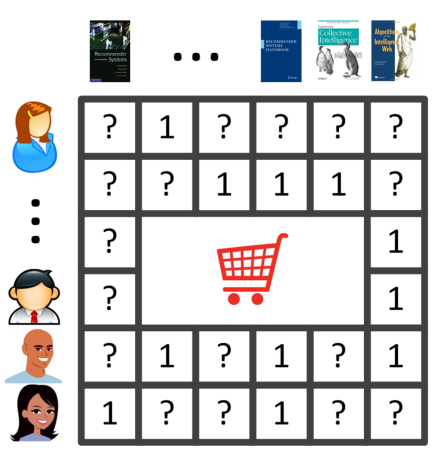
\includegraphics[width=3in]{matrix}
		\caption{user-item 隐式反馈矩阵}
		\label{gra3}
	\end{center}
\end{figure}
在这一节, 我们首先回顾BPR算法,然后讨论它的一些局限性,也就是其收敛缓慢与冷启动问题。通常用户与物品的隐式反馈可以表示为如图\ref{gra3}所示的矩阵, 矩阵的“1”表示用户已经对该物品有过交互行为, 比如购买,点击等, 矩阵的“?”则表示用户还未对该物品有过交互行为。

\subsubsection{Pairwise Preference Assumption}
BPR\cite{rendle2009bpr}是一个应对隐式反馈很流行的推荐框架. 它基于这样一个偏好假设: 如果一个用户$u$已经选择了物品$i$但是没有选择物品$j$,那么在BPR中, 我们认为相对于物品$j$用户$m$更喜欢物品$i$,并定义用户$u$关于物品$i$与$j$的偏好关系为:
\begin{equation}
\label{pairwisepre}
p \left( i \succ_u j \right) := f \left( x_{uij} \right),
\end{equation}
这里$f \left(x\right) = 1/\left(1+exp\left(-x\right)\right)$\footnote{$f \left(x\right)$即为sigmoid函数}, $x_{uij} := s\left(u,i\right) - s\left(u,j\right)$, $s\left(\cdot,\cdot\right)$可以是任何表示用户与物品相关程度的函数。在BPR\cite{rendle2009bpr}中, $s\left(\cdot,\cdot\right)$为用户对物品的预测值, 即$s\left(u,i\right) = \hat{r}_{ui}$, $x_{uij} = \hat{r}_{ui}-\hat{r}_{uj}$.


\subsubsection{预测公式(Prediction Rule)}

在BPR中, 用户$u$对于物品$i$的预测值$\hat{r}_{ui}$公式为:
\begin{equation}
\hat{r}_{ui} = U_{u\cdot}V_{i\cdot}^T + b_i
\end{equation}


\subsubsection{Likelihood of Pairwise Preference}

伯努利分布(Bernouli distribution)是关于布尔变量 $x \in \{0,1\}$ 的概率分布, 其连续参数 $p \in \left[0,1\right]$的概率.
\begin{equation}
\left( x|p \right) = Ber\left(x|p \right)=p^x\left(1-p \right)^{1-x}
\end{equation}

若记事件 $\left(\hat{r}_{ui} > \hat{r}_{uj}\right)$ 的概率为$p\left(\hat{r}_{ui} > \hat{r}_{uj}\right)$, 布尔变量$\delta\left(\left(u,i\right) \succ \left(u,j\right)\right)$ 服从伯努利分布, 那么用户$u$的likelihood of pairwise preference 在\cite{rendle2009bpr}中被定义为:
\begin{equation}
\label{LPP}
\begin{aligned}
LPP_u  
&= \prod_{i,j \ \in \  \mathcal{I}}p\left(\hat{r}_{ui} > \hat{r}_{uj}\right)^{\delta\left(\left(u,i\right) \succ \left(u,j\right)\right)} \left[1-p\left(\hat{r}_{ui} > \hat{r}_{uj}\right)\right]^{1-\delta\left(\left(u,i\right) \succ \left(u,j\right)\right)}\\
&= \prod_{\left(u,i\right) \succ \left(u,j\right)}p\left(\hat{r}_{ui} > \hat{r}_{uj}\right)\prod_{\left(u,i\right) \preceq \left(u,j\right)}\left[1-p\left(\hat{r}_{ui} > \hat{r}_{uj}\right)\right]
\end{aligned}
\end{equation}

这里的$\left(u,i\right) \succ \left(u,j\right)$ 表示用户 $u$ 相比物品 $i$ 更喜欢物品 $j$.

用 $f \left(\hat{r}_{uij} \right)$ 来近似表示概率
$p\left(\hat{r}_{ui} > \hat{r}_{uj}\right)$ \cite{rendle2009bpr}, 对于公式\ref{LPP}取其对数即$\ln LPP_u$, 那么就有:
\begin{equation}
\label{eq5}
\begin{aligned}
\ln LPP_u
&= \ln \prod_{\left(u,i\right) \succ \left(u,j\right)} f \left(\hat{r}_{uij}\right) + \ln \prod_{\left(u,i\right) \preceq \left(u,j\right)}\left[1- f \left(\hat{r}_{uij}\right)\right]\\
&= \ln \prod_{\left(u,i\right) \succ \left(u,j\right)} f \left(\hat{r}_{uij}\right) + \ln \prod_{\left(u,i\right) \succ \left(u,j\right)}\left[1-\left(1- f \left(\hat{r}_{uij}\right)\right)\right]\\
&= \ln \prod_{\left(u,i\right) \succ \left(u,j\right)} f \left(\hat{r}_{uij}\right) + \ln \prod_{\left(u,i\right) \succ \left(u,j\right)} f \left(\hat{r}_{uij}\right)\\
&= 2\ln \prod_{\left(u,i\right) \succ \left(u,j\right)} f \left(\hat{r}_{uij}\right)\\
&= 2 \sum_{i\in\mathcal{I}_u^{tr}}
\sum_{j \in \mathcal{I}\setminus \mathcal{I}_u^{tr}}\ln f \left(\hat{r}_{uij}\right)
\end{aligned}
\end{equation}
在这里$\hat{r}_{uij} = \hat{r}_{ui} - \hat{r}_{uj}$, $f \left(x\right) = 1/\left(1+exp\left(-x\right)\right)$, .

\subsubsection{目标函数}

基于上面的成对偏好假设,可以从隐式反馈数据集中得到所有的偏好集合$D_S := \{\left(u,i,j\right) | v_i \in I_{u}^+ \wedge v_j \in I \setminus I_{u}^+\}$,$I_m^+$表示被用户$u$选择过的物品集合,三元组$\left(u,i,j\right)$表示用户$u$选择过物品$v_i$但是没有选择过物品$v_j$。我们把$v_i$叫做一个positive item,$v_j$叫做一个negative item。对于给定的集合$D_S$, BPR的目标便是最大化所有user-item pair的似然偏好:

\begin{equation}
\label{eq6}
arg \max_{\substack \Theta } \prod_{\left(u,i,j\right) \in D_S} p\left(i \succ_u j\right),
\end{equation}

公式\eqref{eq6}等价于最小化负的对数似然函数:

\begin{equation}
\label{Lfeedback}
L_{feedback} = - \sum_{\left(u,i,j\right) \in D_S}\ln f \left( x_{uij}\right) + \lambda\|\Theta\|^2,
\end{equation}
这里的$x_{uij} = \hat{r}_{uij}$, $\Theta$表示算法中需要学习的模型参数集合,$\lambda$表示超参数集合。在实际的算法学习中, BPR的学习算法经常采用均匀采样的随机梯度下降(\textbf{S}tochastic \textbf{G}radient \textbf{D}escent)进行迭代学习。

更为具体的,公式\eqref{Lfeedback}也就是最小化下面的目标函数(Objective Function): 
\begin{equation}
\label{eq8}
\min_{\substack\Theta}\sum_{u\in\mathcal{U}} \ \sum_{i\in\mathcal{I}_u}\sum_{j\in\mathcal{I}\setminus\mathcal{I}_u}\Phi_{uij}
\end{equation}
这里的
$\Phi_{uij}
= 
- \ln f \left(\hat{r}_{uij}\right) 
+ \frac{\alpha_u}{2}\|U_{u\cdot}\|^2
+ \frac{\alpha_v}{2}\|V_{i\cdot}\|^2
+ \frac{\alpha_v}{2}\|V_{j\cdot}\|^2
+ \frac{\beta_v}{2}\|b_{i}\|^2
+ \frac{\beta_v}{2}\|b_{j}\|^2$, $\Theta = \{U_{u\cdot},V_{i\cdot},b_i\}
$的将要学习的参数集合。


\subsubsection{随机梯度}
对于一个随机采样而得的三元组$\left(u,i,j\right)$, 对目标函数中的参数求其偏导即可得梯度。

在此之前先做一些准备工作,对于函数$f(x) = 1/\left(1+e^{-x}\right)$的导数:

\begin{equation*}
f^{'}(x) = -\frac{1}{\left(1+e^{-x}\right)^2} e^{-x}\left(-1\right) = \frac{e^{-x}}{\left(1+e^{-x}\right)^2} = \frac{1}{\left(1+e^{x}\right)\left(1+e^{-x}\right)} = {f(x)f(-x)}
\end{equation*}

下面开始对参数$U_{u\cdot}$求其偏导:
\begin{equation}
\begin{aligned}
\bigtriangledown U_{u\cdot} 
= \frac{\partial \Phi_{uij}}{\partial U_{u\cdot}}
&=-\frac{\partial \ln f\left(\hat{r}_{uij}\right)}{\partial f\left(\hat{r}_{uij}\right)} 
\frac{\partial f\left(\hat{r}_{uij}\right) }{\partial \hat{r}_{uij}} 
\frac{\partial \hat{r}_{uij}}{\partial U_{u\cdot}}
\ + \  \alpha_uU_{u\cdot}\\
&= -\frac{1}{f\left(\hat{r}_{uij}\right)} 
\frac{\partial f\left(\hat{r}_{uij}\right) }{\partial \hat{r}_{uij}} 
\frac{\partial \hat{r}_{uij}}{\partial U_{u\cdot}}
\ + \  \alpha_uU_{u\cdot}\\
&= -\frac{1}{f\left(\hat{r}_{uij}\right)} 
{f\left(\hat{r}_{uij}\right) f\left(-\hat{r}_{uij}\right)}
\frac{\partial f\left(\hat{r}_{ui} - \hat{r}_{uj}\right) }{\partial U_{u\cdot}} 
\ + \ \alpha_uU_{u\cdot}\\
&= -{f\left(-\hat{r}_{uij}\right)} \frac{\partial f\left[\left(U_{u\cdot}V_{i\cdot}^T+b_i\right) - \left(U_{u\cdot}V_{j\cdot}^T+b_j\right)\right] }{\partial U_{u\cdot}} 
\ + \ \alpha_uU_{u\cdot}\\
&= -{f\left(-\hat{r}_{uij}\right)} \left(V_{i\cdot} - V_{j\cdot}\right)  
\ + \  \alpha_uU_{u\cdot}\\
\end{aligned}
\end{equation}

同样其他参数随机梯度如下:
%\begin{equation}
\begin{align} %align环境不要有空行
\bigtriangledown V_{i\cdot} &= \frac{\partial \Phi_{uij}}{\partial V_{i\cdot}}=-f\left(-\hat{r}_{uij}\right)U_{u\cdot} + \alpha_vV_{i\cdot}\\
\bigtriangledown V_{j\cdot} &= \frac{\partial \Phi_{uij}}{\partial V_{j\cdot}}=-f\left(-\hat{r}_{uij}\right)\left(-U_{u\cdot}\right) + \alpha_vV_{j\cdot}\\
\bigtriangledown b_i        &= \frac{\partial \Phi_{uij}}{\partial b_i} =-f\left(-\hat{r}_{uij}\right)+\beta_vb_i\\
\bigtriangledown b_j        &= \frac{\partial \Phi_{uij}}{\partial b_j} =-f\left(-\hat{r}_{uij}\right)\left(-1\right)+\beta_vb_j
\end{align}
%\end{equation}

\subsubsection{迭代更新}
对于三元组  $\left(u,i,j\right)$ 在采用SGD的BPR算法中的更新公式如下:
%align环境的每行公式默认会进行编号,aligned环境不会
\begin{align}
	\label{eq10}
U_{u\cdot} &= U_{u\cdot} - \gamma\bigtriangledown U_{u\cdot}\\
V_{i\cdot} &= V_{i\cdot} - \gamma\bigtriangledown V_{i\cdot}\\
V_{j\cdot} &= V_{i\cdot} - \gamma\bigtriangledown V_{j\cdot}\\
b_{i\cdot} &= b_i - \gamma\bigtriangledown b_{i}\\
b_{j\cdot} &= b_j - \gamma\bigtriangledown b_{j}
\end{align}

这里的 $\gamma$ 为学习率(learning rate).

\subsubsection{BPR算法}
如算法\ref{al1}即为采用SGD求解的BPR算法。
\IncMargin{1em}
\begin{algorithm}[ht]
	\SetAlgoNoLine %不要算法中的竖线
	\BlankLine
	
	initialize the model parameter $\Theta$\;
	\For {$t_1 = 1,\cdots,T$}{
		\For {$t_2 = 1,\cdots, |\mathcal{P}|$}{
			Randomly pick up a pair $\left(u,v_i\right) \in \mathcal{P}$\;
			Randomly pick up an item $v_j$ from $\mathcal{I} \setminus \mathcal{I}_{u}^+$\;
			Calculate the gradients via Eq.(9-13)\;
			Update the model parameters via Eq.(14-18)\;
		}	
	}
	\caption{The SGD algorithm for BPR}
	\label{al1}%label 放置的位置有讲究, 放后面
\end{algorithm}
\DecMargin{1em}

\subsubsection{收敛缓慢的原因}
由于上面的均匀采样方式会产生很多对于参数学习贡献微弱的train pairs,因此常常会导致收敛缓慢。确切的讲,对于一个给定的训练采样$\left(u,i,j\right) \in D_S$, 由公式\ref{Lfeedback}对随机梯度下降的任意一参数$\theta \in \Theta$求其偏导:

\begin{equation}
\label{eq19}
\frac {\partial L_{feedback}} {\partial\theta} 
= -f\left(-x_{uij}\right)\frac{\partial\left(x_{uij}\right)}{\partial\theta}
= \left(f\left(x_{uij}\right)-1\right) \frac{\partial\left(x_{uij}\right)}{\partial\theta}
\end{equation}

根据公式\eqref{eq19},如果$f \left(x_{uij}\right) \rightarrow +1$,随机梯度将接近于0,则训练采样$\left(u,i,j\right)$对于优化目标的贡献将会变得很小。
\begin{figure}[htbp]
	\begin{center}
		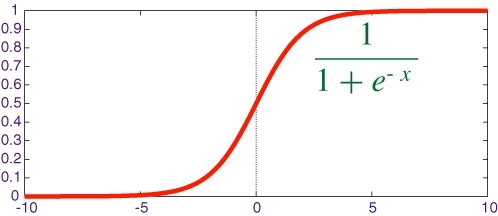
\includegraphics[width=4in]{sigmoid}
		\caption{sigmoid函数$f \left(x\right) $图像}
		\label{gra-sigmoid}
	\end{center}
\end{figure}

联系公式\eqref{eq19}与公式\eqref{pairwisepre},由图\ref{gra-sigmoid} sigmoid函数图像可得, 当$f \left(x_{uij}\right) \rightarrow +1$时, 也就是$x_{uij} = \hat{r}_{ui} - \hat{r}_{uj}$越来越大, 即用户对于物品$v_i$与$v_j$的预测差值越来越大. 因此为了加速学习, 针对一个已有的user-item pair中的物品 $v_i$,要采样的物品$v_j$应当是$v_i$相比有竞争力的物品, 更进一步说也就是由该用户对于$v_i$与$v_j$的偏好得分应该是相近的,否则这个采样对于SGD便是低效的采样。

从经验上来讲,每个用户只会浏览一小部分的物品并对这些浏览过的物品提供一些交互反馈。如果均匀采样器均等地从整个物品集合中采样negative  item.对于一个user-item  pair,大部分均匀采样的物品并不具有可比性或者很难被相关的用户浏览。举个例子,iPhone与牙刷或iPhone与一个冷门的手机品牌可能会经常被均匀采样器采得。而由于这些低效的training pair对于SGD几乎作用很小,整个训练过程便会收敛地极其缓慢。

除此以外,与经典的分解技术相似,如果一个用户或物品缺乏足够的反馈,其对应的隐式表达往往不能够被很好的学习到。在现实世界数据集中,用户行为与物品流行度的分布往往呈现长尾状。这就导致了大部分的用户和物品仅仅有很小部分的反馈数据。此外,在真实的推荐系统中,新的个体可能在任何时间被加入到推荐系统中。因此,BPR框架也很容易受制于冷启动问题。

\subsection{Latent Dirichlet allocation}
Latent Dirichlet allocation(LDA),隐含狄利克雷分布,是一种主题模型(topic model),它可以将文档集中每篇文档的主题按照概率分布的形式给出。同时它是一种无监督学习算法,在训练时不需要手工标注的训练集,需要的仅仅是文档集以及指定主题的数量即可。此外LDA的另一个优点则是,对于每一个主题均可找出一些词语来描述它。

LDA首先由于2003年提出\cite{blei2003latent},目前在文本挖掘领域包括文本主题识别、文本分类以及文本相似度计算方面都有应用。


\subsubsection{数学模型}
LDA是一种典型的词袋(Bag-of-words)模型,即它认为一篇文档(document)是由一组词(word)构成的一个集合,词与词之间没有顺序以及先后的关系。一篇文档可以包含多个主题(topic),文档中每一个词都由其中的一个主题生成。

\begin{figure}[htbp]
	% caption放上面就会显示在图的上方,出现在下面就是出现在图的下方
	% label的位置也有讲究
	\begin{center}
		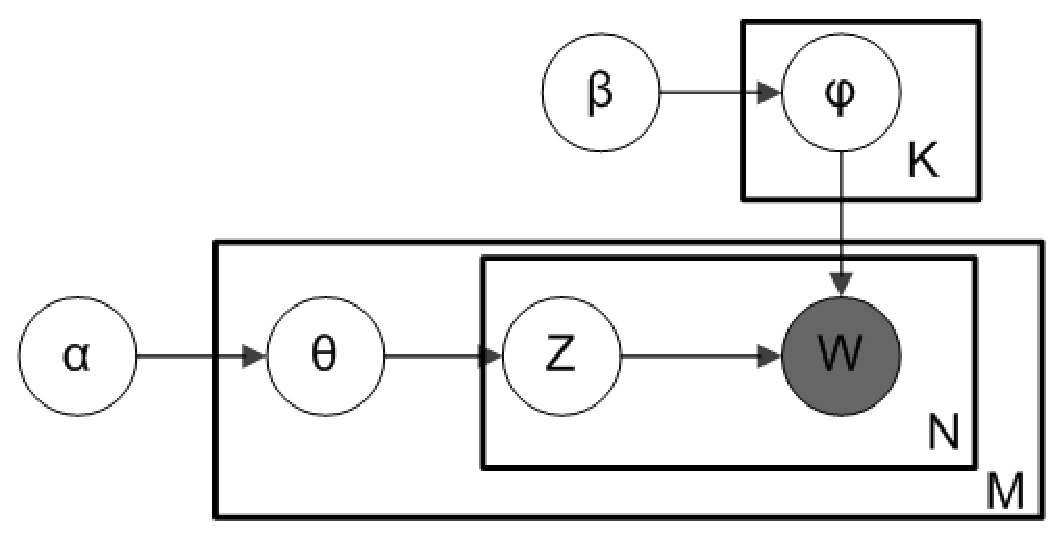
\includegraphics[width=4in]{LDA}
		\caption{LDA 贝叶斯网络结构}
		\label{gra4}
	\end{center}
\end{figure}

另外,正如Beta分布是二项式分布的共轭先验概率分布,狄利克雷分布作为多项式分布的共轭先验概率分布。因此正如图\ref{gra4}, LDA贝叶斯网络结构中所描述的,在LDA模型中一篇文档生成的方式如下:
\begin{itemize}
	\item 从狄利克雷分布$\alpha$ 中取样生成文档$i$的主题分布$\theta_i$
	\item 从主题的多项式分布$\theta_i$中取样生成文档$i$第$j$个词的主题$z_{i, j}$
	\item 从狄利克雷分布$\beta $中取样生成主题$z_{i, j}$的词语分布$\phi_{z_{i, j}}$
	\item 从词语的多项式分布$\phi_{z_{i, j}}$中采样最终生成词语$w_{i, j}$
\end{itemize}
因此整个模型中所有可见变量以及隐藏变量的联合分布是
\begin{equation}
p(w_i, z_i, \theta_i, \Phi | \alpha, \beta) = \prod_{j = 1}^{N} p(\theta_i|\alpha)p(z_{i, j}|\theta_i)p(\Phi|\beta)p(w_{i, j}|\theta_{z_{i, j}})
\end{equation}


最终一篇文档的单词分布的最大似然估计可以通过将上式的$\theta_i$以及$\Phi$进行积分和对$z_i$进行求和得到
\begin{equation}
p(w_i | \alpha, \beta)  = \int_{\theta_i}\int_{\Phi }\sum_{z_i}p(w_i, z_i, \theta_i, \Phi | \alpha, \beta) 
\end{equation}


根据$p(w_i | \alpha, \beta)$ 的最大似然估计,最终可以通过吉布斯采样等方法估计出模型中的参数。


\subsubsection{使用吉布斯采样估计LDA参数}
在LDA最初提出的时候,人们使用EM算法(Expectation-maximization algorithm)进行求解,后来人们普遍开始使用较为简单的Gibbs Sampling,具体过程如下:
\begin{itemize}
	\item 首先对所有文档中的所有词遍历一遍,为其都随机分配一个主题,即$z_{m,n}=k\sim Mult(1/K)$,其中$m$表示第$m$篇文档,$n$表示文档中的第$n$个词,$k$表示主题,$K$表示主题的总数,之后将对应的$n^{\left(k\right)}_m+1$, $n_m+1$, $n^{\left(t\right)}_k+1$, $n_k+1$, 他们分别表示在$m$文档中$k$主题出现的次数,$m$文档中主题数量的和,$k$主题对应的$t$词的次数,$k$主题对应的总词数。
	\item 之后对下述操作进行重复迭代。
	\item 对所有文档中的所有词进行遍历,假如当前文档$m$的词$t$对应主题为$k$,则$n^{\left(k\right)}_m-1$, $n_m-1$, $n^{\left(t\right)}_k-1$, $n_k-1$, 即先拿出当前词,之后根据LDA中topic sample的概率分布sample出新的主题,在对应的$n^{\left(k\right)}_m$, $n_m$, $n^{\left(t\right)}_k$, $n_k$上分别$+1$。
	\begin{equation}
	p(z_i=k|z_{-i},w) \propto k(n^{(t)}_{k,-i}+\beta_t)(n_{m,-i}^{(k)}+\alpha_k)/(\sum_{t=1}^{V}n_{k,-i}^{(t)}+\beta_t)
	\end{equation}
	\item 迭代完成后输出主题--词参数矩阵$\Phi$和文档--主题矩阵$\Theta$
	\begin{align}
	\phi_{k,t}   &=(n_k^{(t)}+\beta_t)/(n_k+\beta_t)  \\
	\theta_{m,k} &=(n_m^{(k)}+\alpha_k)/(n_m+\alpha_k)
	\end{align}
\end{itemize}









\subsection{本章小结}
本章首先介绍了采用SGD求解的Bayesian Personalized Ranking(BPR)推荐算法, 并且对可能导致其收敛缓慢的均匀采样策略做了讨论。然后简要介绍了LDA模型。